\documentclass[tikz,border=8pt]{standalone}
\usepackage{amsmath,amssymb}
\usetikzlibrary{arrows.meta,calc,decorations.markings}

\begin{document}
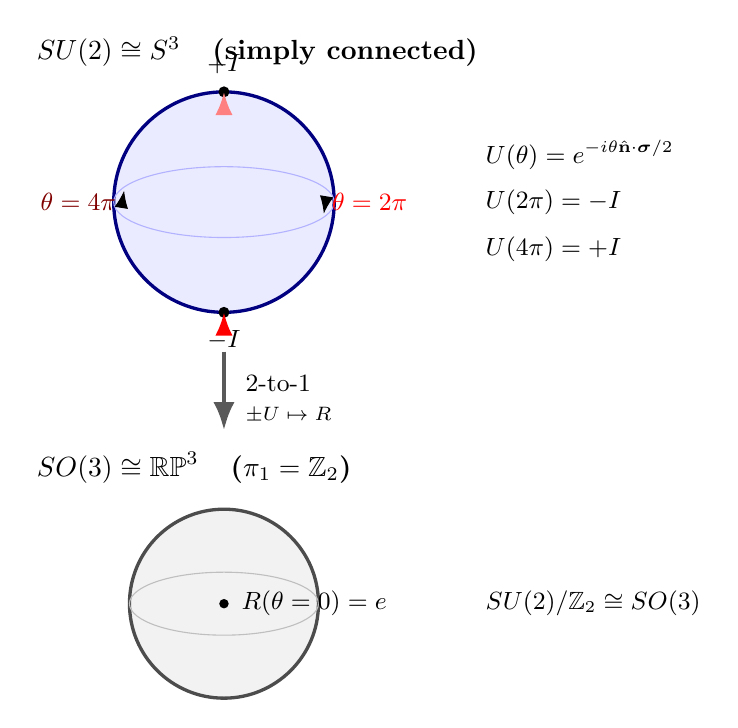
\begin{tikzpicture}[>=Latex]

  % TOP: SU(2) sphere
  \begin{scope}[xshift=0cm, yshift=2.5cm]
    \node[font=\bfseries, anchor=south west] at (-2.5, 1.6) {$SU(2)\cong S^3$\quad(simply connected)};

    \draw[very thick, blue!50!black, fill=blue!8] (0, 0) circle (1.4);
    \draw[blue!30, thin] (0, 0) ellipse (1.4 and 0.45);

    \fill (0, 1.4) circle (0.07);
    \node[anchor=south, font=\small] at (0, 1.5) {$+I$};

    \fill (0, -1.4) circle (0.07);
    \node[anchor=north, font=\small] at (0, -1.5) {$-I$};

    % theta = 2π path: from +I to -I
    \draw[->, very thick, red, decorate, decoration={markings, mark=at position 0.55 with {\arrow{>}}}]
      (0, 1.4) .. controls (1.7, 1.0) and (1.7, -1.0) .. (0, -1.4);
    \node[font=\small, red] at (1.85, 0.0) {$\theta=2\pi$};

    % theta = 4π continues: -I back to +I
    \draw[->, very thick, red!50, dashed, decorate, decoration={markings, mark=at position 0.55 with {\arrow{>}}}]
      (0, -1.4) .. controls (-1.7, -1.0) and (-1.7, 1.0) .. (0, 1.4);
    \node[font=\small, red!50!black] at (-1.85, 0.0) {$\theta=4\pi$};

    \node[font=\small, anchor=west] at (3.2, 0.6) {$U(\theta)=e^{-i\theta\hat{\mathbf n}\cdot\boldsymbol\sigma/2}$};
    \node[font=\small, anchor=west] at (3.2, 0.0) {$U(2\pi)=-I$};
    \node[font=\small, anchor=west] at (3.2, -0.6) {$U(4\pi)=+I$};
  \end{scope}

  % Mapping arrow
  \draw[->, ultra thick, gray!70!black] (0, 0.6) -- (0, -0.4);
  \node[font=\small, anchor=west] at (0.15, 0.2) {2-to-1};
  \node[font=\scriptsize, anchor=west] at (0.15, -0.2) {$\pm U \mapsto R$};

  % BOTTOM: SO(3) ball
  \begin{scope}[xshift=0cm, yshift=-2.6cm]
    \node[font=\bfseries, anchor=south west] at (-2.5, 1.4) {$SO(3)\cong\mathbb{RP}^3$\quad($\pi_1=\mathbb Z_2$)};

    \draw[very thick, gray!60!black, fill=gray!10] (0, 0) circle (1.2);
    \draw[gray!50, thin] (0, 0) ellipse (1.2 and 0.40);

    \fill (0, 0) circle (0.06);
    \node[font=\small, anchor=west] at (0.10, 0) {$R(\theta=0)=e$};

    \node[font=\small, anchor=west] at (3.2, 0.0) {$SU(2)/\mathbb Z_2 \cong SO(3)$};
  \end{scope}
\end{tikzpicture}
\end{document}
